% ==============================================================================
% CHAPTER 6 — Decision Trees
% ==============================================================================
\chapter{Decision Trees}\label{ch:trees}

\begin{intuition}[title=\textbf{Chapter Overview}]
Decision trees partition the feature space into axis-aligned regions via a sequence of binary splits. They are interpretable, handle mixed data types, and require no feature scaling. This chapter derives the splitting criteria (entropy, Gini, variance reduction), presents the CART algorithm, discusses pruning, and covers regression trees.
\end{intuition}

% ==============================================================================
\section{CART Algorithm}
% ==============================================================================

\begin{definition}[Decision Tree]
A decision tree is a function $T : \R^p \to \mathcal{Y}$ defined by a binary tree where each internal node tests a condition $x_j \leq t$ for some feature $j$ and threshold $t$, and each leaf assigns a prediction $\hat{y}$.
\end{definition}

\begin{algorithme}[title=\textbf{CART (Classification and Regression Trees)}]
\begin{enumerate}
    \item Start with the full dataset at the root node.
    \item For each node, find the best split $(j^*, t^*)$:
    \[
        (j^*, t^*) = \argmin_{j,t}\bigl[\frac{n_L}{n}\,Q(R_L) + \frac{n_R}{n}\,Q(R_R)\bigr],
    \]
    where $R_L = \{i : x_{ij} \leq t\}$, $R_R = \{i : x_{ij} > t\}$, and $Q$ is an impurity measure.
    \item Create two child nodes with the subsets $R_L$ and $R_R$.
    \item Recurse on each child until a stopping criterion is met (max depth, min samples, or pure node).
    \item Assign to each leaf the majority class (classification) or mean target (regression).
\end{enumerate}
\end{algorithme}

\begin{remark}
CART uses \emph{greedy} top-down splitting. Finding the globally optimal tree is NP-hard, so the greedy heuristic is standard. Each split considers all $p$ features and $O(n)$ thresholds, giving $O(np)$ cost per node.
\end{remark}

\begin{proposition}[Computational Complexity]
Building a full binary tree has depth $O(\log n)$ to $O(n)$. At each level, all $n$ samples are scanned across $p$ features. Sorting-based splitting achieves $O(np\log n)$ time per level and $O(np\log^2 n)$ overall for balanced trees. The space complexity is $O(n + |T|)$ where $|T|$ is the number of nodes.
\end{proposition}

% ==============================================================================
\section{Splitting Criteria for Classification}
% ==============================================================================

\subsection{Entropy and Information Gain}

\begin{definition}[Shannon Entropy]
For a node with class proportions $\hat{p}_k = \frac{n_k}{n}$, $k = 1,\ldots,K$, the entropy is
\[
    H = -\sum_{k=1}^{K} \hat{p}_k \log_2 \hat{p}_k,
\]
with the convention $0\log 0 = 0$. Entropy is maximised when all classes are equally likely ($H = \log_2 K$) and minimised at $H = 0$ for a pure node.
\end{definition}

\begin{theorem}[Entropy Bounds]
For $K$ classes: $0 \leq H \leq \log_2 K$. Equality on the left holds iff one $\hat{p}_k = 1$; on the right iff $\hat{p}_k = 1/K$ for all $k$.
\end{theorem}

\begin{proof}
Non-negativity follows from $\hat{p}_k \in [0,1]$ so $-\hat{p}_k\log_2\hat{p}_k \geq 0$. The upper bound follows from Jensen's inequality applied to the concave function $f(x) = -x\log_2 x$:
\[
    H = \sum_k f(\hat{p}_k) \leq K\cdot f\!\left(\frac{1}{K}\right) = K\cdot\frac{1}{K}\log_2 K = \log_2 K.
\]
Alternatively, $H \leq \log_2 K$ is equivalent to $D_{\text{KL}}(\hat{p}\,\|\,\text{Uniform}) \geq 0$.
\end{proof}

\begin{definition}[Information Gain]
The information gain from splitting a node $S$ into subsets $S_L$ and $S_R$ is
\[
    \text{IG}(S, j, t) = H(S) - \frac{|S_L|}{|S|}\,H(S_L) - \frac{|S_R|}{|S|}\,H(S_R).
\]
CART selects the split $(j^*,t^*)$ that maximises IG.
\end{definition}

\begin{proposition}[Non-Negativity of Information Gain]
$\text{IG}(S,j,t) \geq 0$ for all splits, with equality iff the class distribution is identical in $S_L$ and $S_R$. This follows from the concavity of entropy (Jensen's inequality).
\end{proposition}

\begin{example}[Computing Information Gain]
Consider a node with 20 samples: 12 positive, 8 negative. Entropy: $H = -\frac{12}{20}\log_2\frac{12}{20} - \frac{8}{20}\log_2\frac{8}{20} \approx 0.971$.

A split sends 10 positive and 2 negative to the left ($n_L=12$), and 2 positive and 6 negative to the right ($n_R=8$):
\begin{align*}
    H(S_L) &= -\tfrac{10}{12}\log_2\tfrac{10}{12} - \tfrac{2}{12}\log_2\tfrac{2}{12} \approx 0.650, \\
    H(S_R) &= -\tfrac{2}{8}\log_2\tfrac{2}{8} - \tfrac{6}{8}\log_2\tfrac{6}{8} \approx 0.811, \\
    \text{IG} &= 0.971 - \tfrac{12}{20}(0.650) - \tfrac{8}{20}(0.811) \approx 0.256.
\end{align*}
\end{example}

\subsection{Gini Impurity}

\begin{definition}[Gini Impurity]
\[
    G = \sum_{k=1}^{K}\hat{p}_k(1-\hat{p}_k) = 1 - \sum_{k=1}^{K}\hat{p}_k^2.
\]
\end{definition}

\begin{proposition}[Gini Properties]
For $K$ classes: $0 \leq G \leq 1 - 1/K$. Gini measures the probability that two randomly drawn samples from the node belong to different classes. For binary classification ($K=2$), $G = 2\hat{p}(1-\hat{p})$.
\end{proposition}

\begin{theorem}[Relationship Between Entropy and Gini]
For binary classification with $\hat{p}_1 = p$, both $H(p) = -p\log_2 p - (1-p)\log_2(1-p)$ and $G(p) = 2p(1-p)$ are concave, symmetric around $p=0.5$, and zero at $p \in \{0,1\}$. A second-order Taylor expansion of $H$ around $p=0.5$ gives $H \approx 1 - \frac{2}{\ln 2}(p-0.5)^2$, which is close to $\frac{1}{\ln 2}G$ after rescaling.
\end{theorem}

\begin{bestpractice}[title=\textbf{Entropy vs.\ Gini}]
\begin{itemize}
    \item In practice, they produce very similar trees (disagreement in $<2\%$ of cases).
    \item Gini is slightly faster to compute (no logarithm).
    \item Entropy tends to produce slightly more balanced splits.
    \item scikit-learn defaults to Gini (\texttt{criterion="gini"}).
\end{itemize}
\end{bestpractice}

\subsection{Comparison of Impurity Measures}

\begin{center}
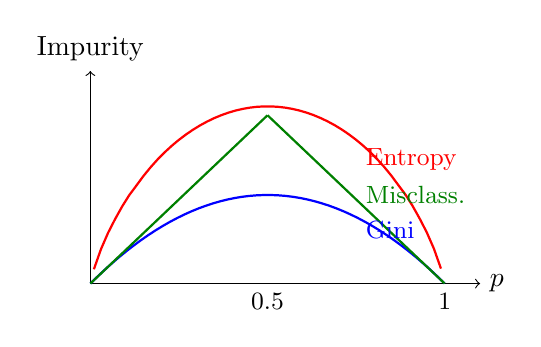
\begin{tikzpicture}[scale=4.5]
    \draw[->] (0,0) -- (1.1,0) node[right] {$p$};
    \draw[->] (0,0) -- (0,0.6) node[above] {Impurity};
    % Gini
    \draw[blue, thick, domain=0:1, samples=50] plot (\x, {2*\x*(1-\x)*0.5});
    % Entropy (scaled)
    \draw[red, thick, domain=0.01:0.99, samples=50]
        plot (\x, {(-\x*ln(\x)/ln(2)-(1-\x)*ln(1-\x)/ln(2))*0.5});
    % Misclassification
    \draw[green!50!black, thick, domain=0:0.5] plot (\x, {\x*0.95});
    \draw[green!50!black, thick, domain=0.5:1] plot (\x, {(1-\x)*0.95});
    % Legend
    \node[blue, right] at (0.75,0.15) {\small Gini};
    \node[red, right] at (0.75,0.35) {\small Entropy};
    \node[green!50!black, right] at (0.75,0.25) {\small Misclass.};
    % Ticks
    \node[below] at (0.5,0) {\small $0.5$};
    \node[below] at (1,0) {\small $1$};
\end{tikzpicture}
\end{center}

\begin{remark}
The misclassification error $1 - \max_k \hat{p}_k$ is not differentiable and not strictly concave, making it unsuitable for greedy splitting (it cannot distinguish between splits that improve purity at different rates). However, it is a valid metric for evaluating the final tree.
\end{remark}

% ==============================================================================
\section{Regression Trees}
% ==============================================================================

\begin{definition}[Regression Tree Impurity]
For regression, the impurity of a node $R$ is the variance of the target values:
\[
    Q(R) = \frac{1}{|R|}\sum_{i \in R}(y_i - \bar{y}_R)^2,
    \qquad \bar{y}_R = \frac{1}{|R|}\sum_{i \in R}y_i.
\]
The prediction at each leaf is $\hat{y} = \bar{y}_R$, the mean of the training targets in that region.
\end{definition}

\begin{proposition}[Optimal Constant Prediction]
For squared loss, the constant $c$ minimising $\sum_{i \in R}(y_i - c)^2$ is $c = \bar{y}_R$. This justifies the use of the mean as the leaf prediction.
\end{proposition}

\begin{theorem}[Variance Reduction]
The reduction in impurity for a split is
\[
    \Delta Q = Q(R) - \frac{|R_L|}{|R|}Q(R_L) - \frac{|R_R|}{|R|}Q(R_R)
    = \frac{|R_L|\cdot|R_R|}{|R|^2}(\bar{y}_{R_L} - \bar{y}_{R_R})^2.
\]
The split maximising $\Delta Q$ separates the node into subsets with maximally different means.
\end{theorem}

\begin{proof}
Expand $Q(R) = \frac{1}{|R|}\sum_i y_i^2 - \bar{y}_R^2$ and apply the same decomposition to $Q(R_L)$ and $Q(R_R)$. Using $\bar{y}_R = \frac{|R_L|}{|R|}\bar{y}_{R_L} + \frac{|R_R|}{|R|}\bar{y}_{R_R}$, algebraic simplification yields the stated result.
\end{proof}

\begin{remark}
The variance reduction formula shows that regression tree splits are equivalent to finding the split that maximises the between-group sum of squares, analogous to a one-way ANOVA.
\end{remark}

% ==============================================================================
\section{Pruning}
% ==============================================================================

\begin{definition}[Cost-Complexity Pruning]
Define the cost-complexity criterion for a subtree $T$ of the full tree $T_0$:
\[
    C_\alpha(T) = \sum_{m=1}^{|T|}\sum_{i \in R_m}(y_i - \hat{y}_{R_m})^2 + \alpha\,|T|,
\]
where $|T|$ is the number of leaves and $\alpha \geq 0$ controls the trade-off between fit and complexity. For each $\alpha$, there is a unique smallest subtree $T_\alpha$ minimising $C_\alpha$.
\end{definition}

\begin{algorithme}[title=\textbf{Minimal Cost-Complexity Pruning}]
\begin{enumerate}
    \item Grow the full tree $T_0$ (no stopping criterion other than pure leaves or minimum node size).
    \item For increasing $\alpha$, compute the sequence of subtrees $T_0 \supseteq T_1 \supseteq \cdots \supseteq \{root\}$ by \emph{weakest-link cutting}: repeatedly remove the internal node whose removal increases the training error the least per removed leaf.
    \item Select $\alpha^*$ via $K$-fold cross-validation.
    \item Return $T_{\alpha^*}$.
\end{enumerate}
\end{algorithme}

\begin{proposition}[Weakest Link Cutting]
For an internal node $t$ with subtree $T_t$, define the effective $\alpha$ at which pruning $t$ becomes worthwhile:
\[
    g(t) = \frac{R(t) - R(T_t)}{|T_t| - 1},
\]
where $R(t)$ is the impurity of node $t$ treated as a leaf and $R(T_t) = \sum_{m \in \text{leaves}(T_t)} R(m)$. At each step, prune the node with the smallest $g(t)$.
\end{proposition}

\begin{warning}[title=\textbf{Overfitting Without Pruning}]
An unpruned tree can achieve zero training error by creating one leaf per training sample. This memorises the data and yields poor generalisation. Controlling tree depth, minimum samples per leaf, or post-hoc pruning are essential. Common hyperparameters: \texttt{max\_depth}, \texttt{min\_samples\_split}, \texttt{min\_samples\_leaf}, \texttt{max\_leaf\_nodes}, \texttt{ccp\_alpha}.
\end{warning}

% ==============================================================================
\section{Advantages and Limitations}
% ==============================================================================

\begin{bestpractice}[title=\textbf{Strengths and Weaknesses of Decision Trees}]
\textbf{Strengths:}
\begin{itemize}
    \item Highly interpretable (``white box'' model).
    \item Handle numerical and categorical features without preprocessing.
    \item Invariant to monotone transformations of features (no need for standardisation).
    \item Capture non-linear relationships and interactions automatically.
    \item Fast training and prediction.
\end{itemize}
\textbf{Weaknesses:}
\begin{itemize}
    \item High variance: small changes in data can produce very different trees.
    \item Axis-aligned splits cannot efficiently represent diagonal boundaries.
    \item Prone to overfitting without regularization (pruning).
    \item Greedy construction does not guarantee global optimality.
\end{itemize}
These weaknesses motivate ensemble methods (bagging, random forests, boosting).
\end{bestpractice}

% ==============================================================================
\section{Tree Diagram}
% ==============================================================================

\begin{center}
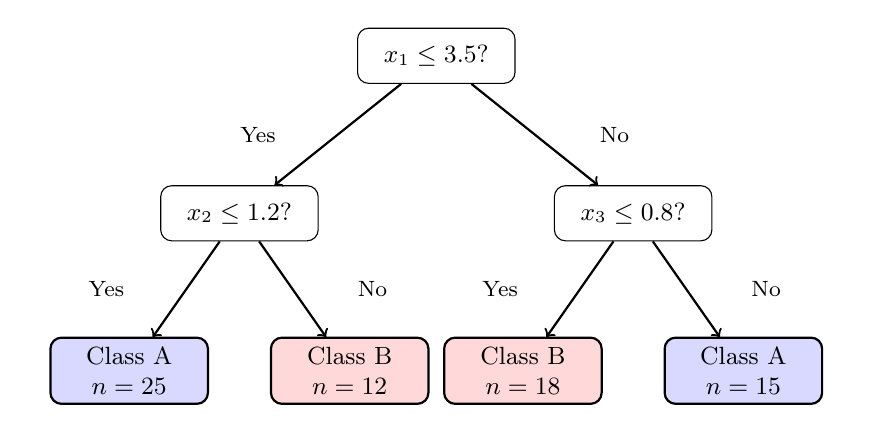
\begin{tikzpicture}[
    level distance=2cm,
    sibling distance=3.5cm,
    every node/.style={draw, rounded corners, minimum width=2cm,
                       minimum height=0.7cm, align=center, font=\small},
    edge from parent/.style={draw, ->, thick},
    level 1/.style={sibling distance=5cm},
    level 2/.style={sibling distance=2.8cm},
]
\node {$x_1 \leq 3.5$?}
    child { node {$x_2 \leq 1.2$?}
        child { node[fill=blue!15] {Class A\\$n=25$}
            edge from parent node[left, draw=none, font=\footnotesize] {Yes} }
        child { node[fill=red!15] {Class B\\$n=12$}
            edge from parent node[right, draw=none, font=\footnotesize] {No} }
        edge from parent node[left, draw=none, font=\footnotesize] {Yes}
    }
    child { node {$x_3 \leq 0.8$?}
        child { node[fill=red!15] {Class B\\$n=18$}
            edge from parent node[left, draw=none, font=\footnotesize] {Yes} }
        child { node[fill=blue!15] {Class A\\$n=15$}
            edge from parent node[right, draw=none, font=\footnotesize] {No} }
        edge from parent node[right, draw=none, font=\footnotesize] {No}
    };
\end{tikzpicture}
\end{center}

% ==============================================================================
\section{Implementation in Python}
% ==============================================================================

\begin{codeblock}[title=\textbf{Decision Tree Classification with scikit-learn}]
\begin{minted}{python}
import numpy as np
from sklearn.datasets import load_iris
from sklearn.model_selection import train_test_split, cross_val_score
from sklearn.tree import DecisionTreeClassifier, export_text, plot_tree
from sklearn.metrics import accuracy_score
import matplotlib.pyplot as plt

X, y = load_iris(return_X_y=True)
feature_names = load_iris().feature_names
X_train, X_test, y_train, y_test = train_test_split(
    X, y, test_size=0.3, random_state=42)

# Train with default settings (no pruning)
tree_full = DecisionTreeClassifier(random_state=42)
tree_full.fit(X_train, y_train)
print(f"Full tree depth: {tree_full.get_depth()}")
print(f"Full tree leaves: {tree_full.get_n_leaves()}")
print(f"Train acc: {tree_full.score(X_train, y_train):.3f}")
print(f"Test acc:  {tree_full.score(X_test, y_test):.3f}")

# Train with pruning constraints
tree_pruned = DecisionTreeClassifier(
    max_depth=3, min_samples_leaf=5, random_state=42)
tree_pruned.fit(X_train, y_train)
print(f"\nPruned tree depth: {tree_pruned.get_depth()}")
print(f"Pruned test acc:   {tree_pruned.score(X_test, y_test):.3f}")

# Print tree rules
print("\nTree rules:")
print(export_text(tree_pruned, feature_names=feature_names))
\end{minted}
\end{codeblock}

\begin{codeoutput}
\begin{minted}{text}
Full tree depth: 5
Full tree leaves: 9
Train acc: 1.000
Test acc:  0.956

Pruned tree depth: 3
Pruned test acc:   0.956

Tree rules:
|--- petal length (cm) <= 2.45
|   |--- class: 0
|--- petal length (cm) >  2.45
|   |--- petal width (cm) <= 1.75
|   |   |--- petal length (cm) <= 4.95
|   |   |   |--- class: 1
|   |   |--- petal length (cm) >  4.95
|   |   |   |--- class: 2
|   |--- petal width (cm) >  1.75
|   |   |--- class: 2
\end{minted}
\end{codeoutput}

\begin{codeblock}[title=\textbf{Cost-Complexity Pruning Path}]
\begin{minted}{python}
# Find optimal alpha via cost-complexity pruning
path = tree_full.cost_complexity_pruning_path(X_train, y_train)
ccp_alphas = path.ccp_alphas

# Train a tree for each alpha and evaluate via CV
cv_scores = []
for alpha in ccp_alphas:
    clf = DecisionTreeClassifier(ccp_alpha=alpha, random_state=42)
    scores = cross_val_score(clf, X_train, y_train, cv=5)
    cv_scores.append(scores.mean())

best_idx = np.argmax(cv_scores)
best_alpha = ccp_alphas[best_idx]
print(f"Best ccp_alpha: {best_alpha:.5f}")
print(f"Best CV accuracy: {cv_scores[best_idx]:.3f}")

# Final model
tree_ccp = DecisionTreeClassifier(
    ccp_alpha=best_alpha, random_state=42)
tree_ccp.fit(X_train, y_train)
print(f"Test accuracy: {tree_ccp.score(X_test, y_test):.3f}")
print(f"Number of leaves: {tree_ccp.get_n_leaves()}")
\end{minted}
\end{codeblock}

\begin{codeblock}[title=\textbf{Visualising the Tree}]
\begin{minted}{python}
fig, ax = plt.subplots(figsize=(14, 6))
plot_tree(tree_ccp, feature_names=feature_names,
          class_names=load_iris().target_names,
          filled=True, rounded=True, ax=ax,
          fontsize=9)
ax.set_title("Cost-Complexity Pruned Decision Tree")
plt.tight_layout()
plt.savefig("decision_tree_plot.pdf")
\end{minted}
\end{codeblock}

\begin{codeblock}[title=\textbf{Regression Tree}]
\begin{minted}{python}
from sklearn.tree import DecisionTreeRegressor
from sklearn.metrics import mean_squared_error

# Synthetic 1D regression data
np.random.seed(42)
X_reg = np.sort(5 * np.random.rand(200, 1), axis=0)
y_reg = np.sin(X_reg.ravel()) + np.random.randn(200) * 0.2

# Fit trees of different depths
fig, axes = plt.subplots(1, 3, figsize=(14, 4))
for ax, depth in zip(axes, [2, 5, 15]):
    reg = DecisionTreeRegressor(max_depth=depth, random_state=42)
    reg.fit(X_reg, y_reg)
    X_plot = np.linspace(0, 5, 500).reshape(-1, 1)
    ax.scatter(X_reg, y_reg, s=10, alpha=0.5, label="Data")
    ax.plot(X_plot, reg.predict(X_plot), "r-", lw=2,
            label=f"depth={depth}")
    mse = mean_squared_error(y_reg, reg.predict(X_reg))
    ax.set_title(f"Depth {depth}, Train MSE={mse:.3f}")
    ax.legend()
plt.tight_layout()
plt.savefig("regression_trees.pdf")
\end{minted}
\end{codeblock}

\begin{codeblock}[title=\textbf{Feature Importance}]
\begin{minted}{python}
# Feature importance from the pruned tree
importances = tree_ccp.feature_importances_
for name, imp in zip(feature_names, importances):
    print(f"  {name:25s}: {imp:.4f}")

# Bar plot
fig, ax = plt.subplots(figsize=(6, 3))
ax.barh(feature_names, importances, color="steelblue")
ax.set_xlabel("Feature Importance (Gini)")
ax.set_title("Decision Tree Feature Importances")
plt.tight_layout()
plt.savefig("tree_importances.pdf")
\end{minted}
\end{codeblock}

\begin{codeoutput}
\begin{minted}{text}
  sepal length (cm)        : 0.0000
  sepal width (cm)         : 0.0000
  petal length (cm)        : 0.4484
  petal width (cm)         : 0.5516
\end{minted}
\end{codeoutput}

% ==============================================================================
\section{Exercises}
% ==============================================================================

\begin{exercise}[Entropy Computation]
A node contains 30 samples: 10 from class A, 12 from class B, 8 from class C. Compute the entropy and Gini impurity. A split sends the 10 A samples and 2 B samples to the left child, and the remaining to the right. Compute the information gain.
\end{exercise}

\begin{exercise}[Gini Derivation]
Prove that for binary classification, the split threshold $t^*$ that minimises the weighted Gini impurity satisfies a condition involving the cumulative class frequencies. Show that the optimal split can be found in $O(n\log n)$ time by sorting the feature values once and scanning.
\end{exercise}

\begin{exercise}[Regression Tree by Hand]
Given the dataset $\{(1, 2.1), (2, 3.8), (3, 4.2), (4, 8.1), (5, 7.9), (6, 9.5)\}$, build a regression tree of depth 2 by hand. At each node, enumerate all possible splits, compute the variance reduction, and select the best.
\end{exercise}

\begin{exercise}[Pruning Experiment]
Using the \texttt{breast\_cancer} dataset:
\begin{enumerate}
    \item Train a full (unpruned) decision tree. Report depth, number of leaves, train/test accuracy.
    \item Plot CV accuracy versus \texttt{ccp\_alpha}.
    \item Select the optimal $\alpha$ and compare the pruned tree with the full tree.
    \item Compare the number of features used by each tree.
\end{enumerate}
\end{exercise}

\begin{exercise}[Instability of Trees]
Decision trees are known for high variance. Generate 10 bootstrap samples from the Iris dataset. Train a decision tree on each and compare the selected root split. How often does it change? Discuss how ensemble methods (bagging, random forests) address this issue.
\end{exercise}

\begin{exercise}[Feature Importance]
scikit-learn computes feature importance as the total reduction in impurity brought by each feature. Formally, for feature $j$:
\[
    \text{Imp}(j) = \sum_{t \in T:\, j(t)=j}\frac{n_t}{n}\Delta Q(t),
\]
where the sum is over all nodes $t$ that split on feature $j$. Train a tree on the Iris dataset, extract \texttt{feature\_importances\_}, and verify the formula by computing it manually from the tree structure using \texttt{tree\_} attributes.
\end{exercise}

\begin{exercise}[Comparison with Other Models]
On the \texttt{wine} dataset, compare a decision tree with logistic regression and $k$-NN:
\begin{enumerate}
    \item Report 5-fold CV accuracy for each method.
    \item For the decision tree, find the optimal \texttt{max\_depth} via CV.
    \item Discuss the interpretability--performance trade-off.
\end{enumerate}
\end{exercise}

\begin{keyformulas}[title=\textbf{Chapter 6 Summary}]
\begin{itemize}
    \item \textbf{Entropy:} $H = -\sum_k \hat{p}_k\log_2\hat{p}_k$
    \item \textbf{Gini:} $G = 1 - \sum_k \hat{p}_k^2$
    \item \textbf{Info Gain:} $\text{IG} = H(S) - \frac{|S_L|}{|S|}H(S_L) - \frac{|S_R|}{|S|}H(S_R)$
    \item \textbf{Regression impurity:} $Q(R) = \frac{1}{|R|}\sum_{i\in R}(y_i - \bar{y}_R)^2$
    \item \textbf{Variance reduction:} $\Delta Q = \frac{n_L n_R}{n^2}(\bar{y}_L - \bar{y}_R)^2$
    \item \textbf{Cost-complexity:} $C_\alpha(T) = \sum_m \text{RSS}_m + \alpha|T|$
    \item \textbf{CART:} Greedy, top-down, binary splits; $O(np\log n)$ per level
\end{itemize}
\end{keyformulas}
